\documentclass{article}
\usepackage[utf8]{inputenc}
\usepackage[T1]{fontenc}
\usepackage{amsmath}
\usepackage{mathtools}
\usepackage{booktabs}
\usepackage{siunitx}
\newcommand{\ui}[2]{#1_{\text{#2}}}

%%-------------------------------------------------------
% MACRO for tikz picture. DO NOT CHANGE ANYTHING !!!!!
\usepackage{tikz}
\usepackage{pgfkeys}
\usepackage{calc}
\usepackage{pgfplots}
\usetikzlibrary{arrows}
\usetikzlibrary{calc}
\usepgflibrary{arrows}
\usetikzlibrary{positioning}
\usetikzlibrary{intersections}
\pgfplotsset{compat=newest}
\usetikzlibrary{shapes.geometric}
\usetikzlibrary{decorations.pathreplacing}
\usetikzlibrary{patterns,decorations.pathmorphing,decorations.markings}
\usetikzlibrary{external}
\usetikzlibrary{plotmarks}
\usetikzlibrary{arrows.meta}
\usepgfplotslibrary{patchplots}
\usepackage{grffile}
\usepgfplotslibrary{fillbetween}
\tikzexternalize

%\newcommand{\includetikz}[1]{%
%	\tikzifexternalizing{%
%		\def\DOIT{1}%
%	}{%
%		\IfFileExists{#1.pdf}{%
%			\includegraphics[scale=1]{#1.pdf}%
%			\def\DOIT{0}%
%		}{%
%			\def\DOIT{1}%
%		}%
%	}%
%	%
%	\if1\DOIT
%	%	\tikzsetnextfilename{mypic_#1}%
%	\tikzsetnextfilename{#1}
%	%   \filemodCmp{#1.tikz}{external/#1.log}%
%	%  {\tikzset{external/force remake=true}\input{#1.tikz}}
%	\input{#1.tikz}
%	\fi
%}

\title{Model of the Mass-Spring-Damper System}
\author{Martin Klau\v{c}o}

\begin{document}
\maketitle

Dynamics of the first mass point is given by
\begin{equation}
	\label{eq:msd:1}
	M_1\ddot{p}_1 - C_1(\dot{p}_2 - \dot{p}_1) - K_1(p_2-p_1) = F_1,
\end{equation}
while the movement of the subsequent mass points are expressed as,
\begin{equation}
	\label{eq:msd:i}
		M_i\ddot{p}_i - C_i(\dot{p}_{i+1} - \dot{p}_i) + C_{i+1}(\dot{p}_i - 
		\dot{p}_{i-1})- K_i(p_{i+1} - p_i) + K_{i-1}(p_i - p_{i-1}) = 0,
\end{equation}
and the dynamics of the last mass point is given by
\begin{equation}
	\label{eq:msd:N}
		M_{N}\ddot{p}_{N} - C_{N-1}(\dot{p}_{N} - 
	\dot{p}_{N-1}) + 	K_{N}(p_{N}-p_{N-1}) = 0.
\end{equation}

Notation:

\begin{tabular}{lcr}\toprule
	Quantity & Symbol & Units \\ \midrule
	mass & $M$ & \SI{}{\kilogram} \\
	spring stiffness & $K$ & \SI{}{\newton\per\meter} \\
	damper coefficient & $C$ & \SI{}{\kilogram\per\second} \\
\bottomrule
\end{tabular}

\begin{figure}
\centering
{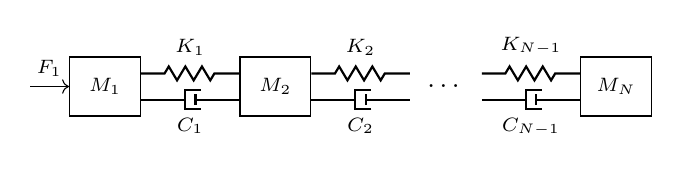
\begin{tikzpicture}
\tikzstyle{spring}=[thick,decorate,decoration={zigzag,pre length=0.3cm,post 
length=0.3cm,segment length=6}]
\tikzstyle{damper}=[thick,decoration={markings,  
  mark connection node=dmp,
  mark=at position 0.5 with 
  {
    \node (dmp) [thick,inner sep=0pt,transform shape,rotate=-90,minimum 
    width=6pt,minimum height=3pt,draw=none] {};
    \draw [thick] ($(dmp.north east)+(2pt,0)$) -- (dmp.south east) -- 
    (dmp.south west) -- ($(dmp.north west)+(2pt,0)$);
    \draw [thick] ($(dmp.north)+(0,-2pt)$) -- ($(dmp.north)+(0,2pt)$);
  }
}, decorate]
	\node [draw, minimum width = 0.9cm, minimum height = 0.75cm] (M1) 
	{\scriptsize$M_1$};
	\node [draw, minimum width = 0.9cm, minimum height = 0.75cm, right = 1.25cm 
	of 
	M1] (M2) {\scriptsize$M_2$};
	\node [minimum width = 0.9cm, minimum height = 0.75cm, right = 1.25cm 
	of 
	M2] (M3) {$\dots$};
	\node [draw, minimum width = 0.9cm, minimum height = 0.75cm, right = 1.25cm 
	of 
	M3] (M4) {\scriptsize$M_{N}$};
	
	% inputs
	\draw [<-] (M1.180) --node [above] {\scriptsize$F_1$}  ++(-0.5cm, 0);
%	\draw [<-] (M4.0) --node [above] {\scriptsize$F_2$}  ++(+0.5cm, 0);
	
	% dampers
	\draw [spring] (M1.20) -- node [above, yshift = +0.1cm] 
	{\scriptsize$K_1$}($(M2.north west)!(M1.20)!(M2.south west)$);
	\draw [damper] (M1.340) -- node [below, yshift = -0.1cm] {\scriptsize$C_1$} 
	($(M2.north 
	west)!(M1.340)!(M2.south west)$);
	
	% dampers
	\draw [spring] (M2.20) --node [above, yshift = +0.1cm] 
		{\scriptsize$K_2$} ($(M3.north west)!(M2.20)!(M3.south west)$);
	\draw [damper] (M2.340) -- node [below, yshift = -0.1cm] {\scriptsize$C_2$} 
	($(M3.north west)!(M2.340)!(M3.south west)$);
	
	% dampers
	\draw [spring] (M3.20) --node [above, yshift = +0.1cm] 
		{\scriptsize$K_{N-1}$} ($(M4.north west)!(M3.20)!(M4.south west)$);
	\draw [damper] (M3.340) --  node [below, yshift = -0.1cm] 
	{\scriptsize$C_{N-1}$} ($(M4.north west)!(M3.340)!(M4.south west)$);
\end{tikzpicture}}
\caption{Scheme of $N$ mass points inter-connected with spring with 
stiffness $K_i$ and dampers $C_i$, for $i \in {1, \ldots, N}$.}
\label{fig:msd}
\end{figure}

\end{document}